\documentclass[onecolumn, draftclsnofoot,10pt, compsoc]{IEEEtran}

\usepackage{graphicx}
\usepackage{url}
\usepackage{setspace}
\usepackage{geometry}
\usepackage{listings}
\usepackage{etoolbox}
\usepackage{pdflscape}

\patchcmd{\thebibliography}{\section*{\refname}}{}{}{}

\geometry{textheight=9.5in, textwidth=7in}

% 1. Fill in these details
\def \CapstoneTeamName{			              			 PlanteR-GB}
\def \CapstoneTeamNumber{					           			 Group 64}
\def \GroupMemberOne{				           				Austin Hodgin}
\def \GroupMemberTwo{				           				Travis Hodgin}
\def \GroupMemberThree{			            Maximillian Schmidt}
\def\GroupMemberFour{		        	               Zach Lerew}
\def \CapstoneProjectName{	      	    Winter is Coming...}
\def \CapstoneSponsorCompany{		    Oregon State University}
\def \CapstoneSponsorPerson{		 			  				 Victor Hsu}

% 2. Uncomment the appropriate line below so that the document type works
\def \DocType{		%Problem Statement
				%Requirements Document
				%Technology Review
				Design Document
				%Progress Report
				}

\newcommand{\NameSigPair}[1]{\par
\makebox[2.75in][r]{#1} \hfil 	\makebox[3.25in]{\makebox[2.25in]{\hrulefill} \hfill		\makebox[.75in]{\hrulefill}}
\par\vspace{-12pt} \textit{\tiny\noindent
\makebox[2.75in]{} \hfil		\makebox[3.25in]{\makebox[2.25in][r]{Signature} \hfill	\makebox[.75in][r]{Date}}}}
% 3. If the document is not to be signed, uncomment the RENEWcommand below
\renewcommand{\NameSigPair}[1]{#1}

%%%%%%%%%%%%%%%%%%%%%%%%%%%%%%%%%%%%%%%
\begin{document}
\begin{titlepage}
    \pagenumbering{gobble}
    \begin{singlespace}
    	%\includegraphics[height=4cm]{coe_v_spot1}
        \hfill

        % 4. If you have a logo, use this includegraphics command to put it on the coversheet.
        
\includegraphics[height=4cm]{logo.png}

        \par\vspace{.2in}
        \centering
        \scshape{
            \huge CS Capstone \DocType \par
            {\large\today}\par
            \vspace{.5in}
            \textbf{\Huge\CapstoneProjectName}\par

            %\vfill
						\vspace{1in}

            {\large Prepared for}\par
            \Huge \CapstoneSponsorCompany\par
            \vspace{5pt}
            {\Large\NameSigPair{\CapstoneSponsorPerson}\par}

						\vspace{1in}

            {\large Prepared by}\par
						{\huge \CapstoneTeamNumber}\par
            \CapstoneTeamName\par
            \vspace{5pt}

            {
							\Large
							\NameSigPair{\GroupMemberOne}\par
							\NameSigPair{\GroupMemberTwo}\par
							\NameSigPair{\GroupMemberThree}\par
							\NameSigPair{\GroupMemberFour}\par
            }

            \vspace{20pt}
        }
%\textbf{\textsuperscript{citation needed}}
				\newpage
        \begin{abstract}
				\noindent This document details the entire system design for the PlanteR-GB system
        \end{abstract}
    \end{singlespace}
\end{titlepage}

\newpage

\pagenumbering{arabic}
\tableofcontents
% 7. uncomment this (if applicable). Consider adding a page break.
%\listoffigures
%\listoftables
\clearpage
\singlespace

\newpage

% Document outline based on summary of IEEE 1016-2009 from http://www.zeynepaltan.info/SDD-Template.pdf

	% Introduction
	\section{Introduction}
		\subsection{Purpose}
		\subsection{Scope}
		\subsection{Overview}
		\subsection{Definitions and Acronyms}
		\subsection{Reference Material}
			\begingroup
				\renewcommand{\addcontentsline}[3]{}% Remove functionality of \addcontentsline
				\renewcommand{\section}[2]{}% Remove functionality of \section
				%\cite[Sec 3.8]{sourceName}
				\bibliography{ref}
				\bibliographystyle{IEEEtran}
			\endgroup

	\section{System Overview}
		\subsection{Assumptions}
		\subsection{General Constraints}
		\subsection{System Environment}


	\section{System Architecture}
		\subsection{System Diagram}
		NOTE:TO BE REPLACED WITH REAL DIAGRAM
		
		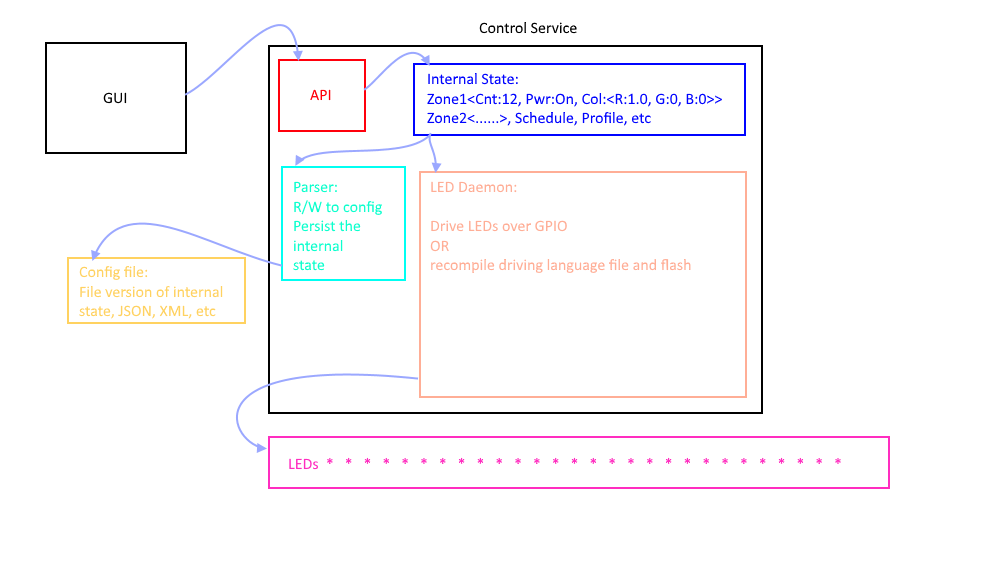
\includegraphics[width=\linewidth]{sysdiag.png}

		\subsection{Hardware}
			\subsubsection{Master Controller}
			\subsubsection{Slave Controller}
		\subsection{Control Service}
			\subsubsection{API}
			\subsubsection{Internal State}
			\subsubsection{Data Parser}
		\subsection{Data Design}
			\subsubsection{Data Description}
			\subsubsection{Zones table}
			\subsubsection{Schedules table}
			\subsubsection{Profiles table}
			\subsubsection{Controllers table}
		\subsection{LED Control System}
			\subsubsection{Slave Controller Communication}
			\subsubsection{Slave Controller Software}


	\section{Human Interface Design}
		\subsection{Overview of User Interface}
		\subsection{Command Line Interface}
			\subsubsection{Interface Overview}
			\subsubsection{Mockup}
		\subsection{Web Interface}
			\subsubsection{Interface Overview}
			\subsubsection{Home Page}
			\subsubsection{Mockup}
			\subsubsection{Zones Page}
			\subsubsection{Mockup}
			%... etc for more pages

	%\section{Requirements Matrix} %??? What is this, it was in a template somewhere

	\section{Appendices} % OR glossary??



\end{document}
